The last two chapters covered methodological guidelines for variability as well
as version assessment. While those two terms, \emph{variability} and
\emph{versions} represent two orthogonal dimensions of a configurable software
systems’ evolution history. To provide a closed description of guidelines for performance
evolution assessment, this chapter finally presents a guideline to assessing
performance for a given variant and version. In Figure~\ref{fig:roadmap_3}, we
present the methodological roadmap and questions to be answered in this chapter.

\begin{figure}[h!]
	\centering
	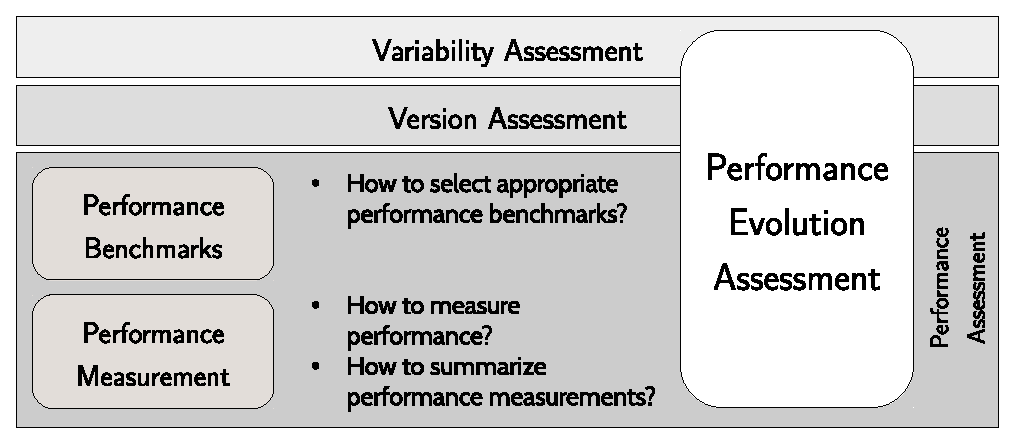
\includegraphics[width=0.9\textwidth]{images/process_perfassessment.eps}
	\caption{Methodological road-map: performance assessment}
	\label{fig:roadmap_3}
\end{figure}

First, in section we categorize software systems with respect to the availability of suitable performance
benchmarks; second, we outline the general properties of profiling tool support
used throughout dynamic program analysis; finally, we discuss different statistical
with respect to their applicability in the context of performance assessment
and robustness.

\section{Performance Benchmarks}
The essential part of assessing performance for a software system is the choice
of a benchmark that one wants to evaluate the software against. For the choice
of a suitable benchmark, two consecutive questions need to be answered. First of
all, we need to specify, what aspects of performance we intend to evaluate for
our software system. As presented earlier in chapter 2, the term performance is
generic as it is commonly outlined by different key performance indicators. For
instance, for a web shop application, good performance is characterized by low response
time and high availability, while for file compression, one might rather
conceive high throughput as good performance. That is, given a specific
aspect of performance, i.e., one or more KPIs, for a software system, from
testing against a suitable performance benchmark one needs to be able to judge
whether the specified performance goals are met, or not.

Next, once we have specified performance indicators fitting our software system,
we need to select a benchmark, i.e., a repeatable task for the software system
for which we can evaluate performance. To keep performance measurements
comparable throughout all versions and variants, it is required to use
only one benchmark per assessment. Following this principle, and to even compare different software
systems, practitioners are advised to refer to reusable, or more general
performance benchmarks whenever possible. To illustrate this, we can divide
software systems into three general categories for which we are presenting
separate strategies.

First, in the the easiest case, a software system provides software tests, or
performance benchmarks, to use for performance assessment. The idea of using an
existing test suite to assess performance is straightforward and has already
been applied to detect performance regression
\citep{foo_mining_2010,heger_automated_2013}.

Second, a software system can offer functionality for a domain, where
standardized benchmarks have been established, or are commonly used to compare
performance measurements. For instance, for the domain of file compression
there exists a long tradition of using standardized file sets as performance
benchmarks, such as the Canterbury
or Calgary corpus\footnote{See
\url{http://corpus.canterbury.ac.nz/descriptions/} for a detailed 
description.}; for video encoding, the
xiph.org\footnote{\url{https://media.xiph.org/}} foundation provides a large set of video benchmark files; and, more general, for processors the Standard
Performance Evaluation Corporation provides (SPEC) standardized benchmarks for
floating point operations. Whenever a software system falls under a domain for
which standardized benchmarks exist, we advocate to use those.

Finally, if neither a performance benchmark or test suite is available for a
software system, nor domain-specific benchmarks exist, the task of designing a
benchmark is left to the practitioner evaluating the software. As the
conception of performance is generic and highly context-dependent, there is no
standardized recipe for designing a performance benchmark. However, the main
criteria to be satisfied include \emph{expressiveness}, \emph{cost-efficiency}
and \emph{reproducibility}. First, a suitable performance benchmark should
clearly express what a desirable and unfavorable performance measurement is, given a specified
key performance indicator. For instance, if we evaluate performance in terms of
response, or execution time, minimal measurements are desirable. Second, effort
that is required to evaluate a software with a benchmark must be reasonable.
Since performance measurements are usually repeated to decrease measurement
bias, or used for different variants and revisions, performance benchmarks
should be limited in terms of size. However, a performance benchmark needs to
be large enough to sketch performance changes or deviations. Finally, the
construction of a benchmark must be reproducible, i.e., transparent and
plausibly designed as the overall value of a performance benchmark depends on
whether we can draw any conclusion from performance measurements obtained from
it.

In conclusion, for the context of our methodology, the advocated guideline for
selecting and designing a performance benchmark for a configurable software
system is to select a benchmark as generic as possible. If there is no reusable
benchmark available, the design of any performance benchmark should follow the
criteria of expressiveness, cost-efficiency, and reproducibility.

\section{Profiling}
With a software system along with a benchmark set up, the only choice left
before assessing performance is to select a means to obtain and collect
performance measurements. For this type of tool support for dynamic analysis,
commonly referred to as profilers, exists a variety of solutions, varying in
functionality and scope of application.

\cite{satapathy_survey_2015} have surveyed a selection of profilers for dynamic
analysis. The authors categorize their selection into three categories,
including VM-profiling-based, instumentation-based, and profilers based on
aspect-oriented programming (AOP). While for VM-based profilers, make use of
profiling functionality offered by the respective platform, such as the Common
Language Interface (CLI) for the family of .NET languages,  or the Java Virtual
Machine (JVM), instrumentation-based profilers add instructions to the software
to the software’s codebase at compilation using instrumentation preprocessors,
or to the software’s executables. AOP-based profilers accommodate profiling
functionality in separate modules called aspects. An aspect’s code, called
advise is executed whenever a corresponding event, called join point,  occurs,
for instance a call of a function that one would like to measure performance
for. Several join points can be summarized by a set of join points, called
point cut. While VM-based profilers are limited to a family of programming
languages, and, as well as instrumentation-based, usually introduce a run-time
overhead that might dilute performance measurements. In contrast to that,
AOP-based profilers  usually perform better, yet are limited to the code base as aspects
are woven into the codebase during re-compilation. Moreover, they require a
higher level of expertise to design and deploy a performance test setup
compared to the former two categories \citep{satapathy_survey_2015}. In addition
to the aforementioned profiler categories, statistical profilers such as
\emph{Performance Counters for
Linux}\footnote{See
\url{http://man7.org/linux/man-pages/man1/perf-stat.1.html} for further
information on \texttt{perf}.}, or \emph{perf}, monitor a software system
performance, for instance hardware counters for regular intervals, and therefore provide an approximation of the software system’s performance with less overhead than instrumentation-based profilers.

In the context of our methodology, we are advocating the use of the unix
command \texttt{time}\footnote{See
\url{http://man7.org/linux/man-pages/man1/time.1.html} for the man page of
\texttt{time} and provided performance metrics to record.} to measure execution
time along with a number of further performance metrics for a software system.
The command is contained in most Linux distributions and, from a black-box
perspective, provides sufficient functionality to sketch performance in terms of
metrics for execution time, memory consumption, or I/O statistics. While tools falling under the aforementioned categories are powerful tools for dynamic analysis and program
optimization, time provides a basic, yet exhaustive support for assessing
performance for software system run on a single host machine. 

\section{Statistical Considerations}\label{sec:statistical_considerations}
In this section, we now discuss the appropriate statistical means to summarize,
compare and interpret measurement results. For the remainder of this section, we
will refer to the following two scenarios. First, to obtain robust results, the
assessment of a single variant needs to be repeated multiple times.
Consequently, to report a single result per metric, the measurements for a
single variant need to be summarized. Second, the assessment of performance for
a variant may comprise several use cases, for instance file
compression and decompression for a compression software. Therefore, performance measures
aggregated from different benchmarks need to be summarized accurately. 

\subsection{Measures of Central Tendency}
For each test run of a software system or variant, we obtain a single-valued
measurement per performance metric. Since we repeat each test run $n$ times
per variant, we obtain a data record $X$ with $n$ measurements $X = X_1, X_2,
\ldots, X_{n-1}, X_n$. While the arithmetic mean is commonly considered the
right way to summarize data records and report a representative average
value, we need to be more cautious with how to summarize data records
\citep{fleming_how_1986,smith_characterizing_1988}. From a statistical
perspective, the intention of summarizing a data record is to find a measure of
central tendency what is representative for the data record.
While the arithmetic mean is an appropriate method for many cases, there exist
other means to summarize data records. Moreover, there exist a number of
criteria for when to use which means to summarize a data record. 

The first question when summarizing a data
record is to ask what the data actually describe and what we intend to express
with our summary. For a data record $X$, we can define a
relationship we would like to conserve while replacing each single $X_i$ with an
average value $\bar{x}$. Based on this relationship, we can derive the
appropriate method to summarize our record. For instance, our data record $X$
describes the time elapsed for a test case and we want the keep the following
relation, saying that the sum of all measurements $\sum_{i = 1}^{n} X_i$ is
equal to the total time elapsed $T$, defined as

$$
T = \sum_{i = 1}^{n} X_i = \sum_{i = 1}^{n} \bar{x}.
$$

Based on the term above, we can derive the definition of the method
appropriate to summarize our data record with respect to the conserved relation
what is the \emph{arithmetic mean}, defined as

\begin{equation} \label{eq:arithmetic_mean}
\begin{split}
\bar{x} = \frac{1}{n} \sum_{i = 1}^{n} X_i.
\end{split}
\end{equation}

Consider another example, similar to the one above, where the test
case is a load test with a predefined number of users and the measurements $X =
X_1, X_2, \ldots, X_{n-1}, X_n$ are
measured as hits per second. Again, we have different measurements we want to
summarize with respect to a relation to conserve. Each user drops the same
number of requests $T$, whereby the hit rate $X_i$ and the respective elapsed
time $t_i = \frac{T}{X_i }$ vary. We now conserve the relationship that the
total number of requests for the data record is the sum of all hit rates $X_i$
times the time elapsed $t_i$. Therefore, we want to substitute each hit rate
$X_i$ with an average value $\hat{x}$ so that the aforementioned relationship is
conserved:

$$
n\cdot T - \sum_{n}^{i=1} X_it_i = 0 \Leftrightarrow n\cdot T - \hat{v}
\sum_{n}^{i=1} t_i = 0 \Leftrightarrow n = \hat{x} \sum_{n}^{i=1} \frac{1}{X_i}
$$

Similar to Eq. \ref{eq:arithmetic_mean} we can derive the definition for the summarization
method to use from the equation above what is the \emph{harmonic mean}, defined as

\begin{equation} \label{eq:harmonic_mean}
\begin{split}
\hat{x} = n \cdot \bigg(\sum_{i=1}^{n} \frac{1}{X_i}\bigg)^{-1} =
\frac{n}{\frac{1}{X_1} + \frac{1}{X_2} + \ldots +
\frac{1}{X_{n-1}} + \frac{1}{X_n}}.
\end{split}
\end{equation}

We see that the summarization methods presented in Eq. \ref{eq:arithmetic_mean}
and \ref{eq:harmonic_mean} are useful for different types of data records, and
should be used accordingly. The arithmetic mean is suitable for records, where the total sum of single
measurements has a meaning, whereas the harmonic mean is suitable for measured
rates or frequencies \citep{smith_characterizing_1988}.

While the aforementioned measures of central tendency should be appropriate for
most cases, they are not always the best choice though since the arithmetic
and harmonic mean are heavily influenced by extreme observations
\citep{shanmugam_statistics_2015}. 
For instance, for the data record $X = 1, 2, 3, 30$, three of four values are
smaller than the arithmetic mean $\bar{x} = 9$. One option is to explicitly exclude outlier
values from the data record. The so-called \emph{trimmed mean} is
obtained by truncating a upper and/or lower percentage $t$ of the data record
and, consequently, computing the (arithmetic or harmonic) mean for the remaining
data record \citep{shanmugam_statistics_2015}. 

While this method is suitable to omit the effects of outliers, one still needs to specify
which upper and/or lower percentage $t$ needs to be truncated. Moreover, the use
a (trimmed) mean requires the data records' frequencies to be distributed
symmetrically around its mean.
A probability distribution is skewed (and therefore asymmetric) if, graphically speaking, its histogram is not
symmetric around its measure of central tendency. A simple method to measure the
skewness of a probability distribution is \emph{Bowley's measure}
\citep{shanmugam_statistics_2015}, defined as

\begin{equation} \label{eq:bowley}
\begin{split}
B_S = \frac{(Q_3 - M) - (M - Q_1)}{Q_3 - Q_1} = \frac{(Q_3 + Q_1 - 2M)}{Q_3
- Q_1},
\end{split}
\end{equation}

where $Q_1$ and $Q_3$ denote the first and third quartile, and $M$ denotes the
median of the probability distribution. The quartiles $Q_i$ with $i \in \left\{
1,2,3 \right\}$ are defined as the values of a data record $X$, so that
$\frac{i}{4}$ of the values of $X$ are smaller than $Q_i$. The \emph{median} is
defined as $Q_2$, i.e., a value $M \in X$ so that half of the values in $X$ are smaller than $M$.

The median itself is a more robust measure of central tendency than the
aforementioned ones since it is less influenced by outliers and can be used for
both skewed and symmetric data records \citep{shanmugam_statistics_2015}. For a
given ascendingly ordered data record $X = X_1, X_2, \ldots, X_{n-1}, X_n$, we
can compute the median as follows:

\begin{equation} \label{eq:median}
\mathrm{Median}(X) = \begin{cases}
     X_{\frac{n+1}{2}} & \text{if $n$ is odd} \\
     \frac{1}{2}\big(X_{\frac{n}{2}} + X_{\frac{n}{2}+1}\big) & \text{if $n$ is
     even}
   \end{cases}~\text{with $X_i \leq X_j$ and $i < j \leq n$ }
\end{equation}

\subsection{Measures of Dispersion}

Last, we take a look at different measures of spread or dispersion. Most
commonly used are the \emph{variance} $\sigma^2$ and the \emph{standard
deviation} $\sigma = \sqrt{\sigma^2}$ defined along the mean $\mu$ of a
probability distribution as

\begin{equation} \label{eq:variance}
\begin{split}
\sigma^2 = \frac{\sum_{i=1}^{n}(X_i - \mu)^2}{n}
\end{split}
\end{equation}

Similar to the (arithmetic or harmonic) mean, the variance and the standard
deviation are heavily influenced by extreme observations
\citep{shanmugam_statistics_2015} and not the best choice in all cases. Instead,
two more robust measures are the \emph{median absolute deviation} (MAD) and the \emph{inter-quartile range} (IQR). The MAD is defined as the median of the absolute deviations from the probability distributions'
median \citep{molyneaux_art_2014}, or, defined as follows:

\begin{equation} \label{eq:mad}
\begin{split}
\mathrm{MAD}(X) = \mathrm{Median}\big(|X - \mathrm{Median}(X)|\big)
\end{split}
\end{equation}
 
The IQR, however, defines the range between the first and the third quartile,
$Q_1$ and $Q_3$ \citep{shanmugam_statistics_2015}. This range is larger for a
widespread data record and smaller for a data range with a narrow spread, but is not influenced by extreme
observations as those outliers do not lie within the range $\left[ Q_1,Q_3
\right] $. The IQR is defined as 

\begin{equation} \label{eq:iqr}
\begin{split}
\mathrm{IQR}(X) = Q_3 - Q_1.
\end{split}
\end{equation}

\subsection{When to use which measure?}
In this section we discussed the arithmetic and harmonic mean as well as the
median as a measure of central tendency, the symmetric property that is
required to use the arithmetic or harmonic mean, and different measures of
spread for a given data record. At the beginning, we have raised the question of how to
summarize data records (a) for an experiment repeated multiple times, and (b)
obtained from different benchmarks. While for case (b) the answer is to use the
arithmetic or harmonic mean (depending on the quality of the measurements), for
(a) the answer is a little more elaborate.

The arithmetic (or harmonic) mean can be used whenever the quality of the
measurement is appropriate and the data record is symmetric. According to
\cite{shanmugam_statistics_2015}, the arithmetic mean is preferable ``when the numbers combine
additively to produce a resultant value'', such as time periods or memory sizes, whereas
the harmonic mean is preferable ``when reciprocals of several non-zero numbers
combine additively to produce a resultant value'', such as rates or frequencies
\citep{smith_characterizing_1988}.
The median is a less precise estimator than the both means, yet more robust
with regard to extreme observations. In addition, the MAD or IQR provide a more
robust means of spread than the standard deviation.

\section{Summarization Strategies}
Besides the statistical considerations regarding the summarization of
performance measurements, we are also challenged by the dimensionality of our
performance evolution history. Given a record of performance measurements for a
number of versions across different variants, we require statistical and
numerical means to summarize performance evolution with single values. For this
purpose, we propose two metrics addressing the following two aspects. First,
different variants usually exhibit different levels of performance
measurements, aside from evolution and fluctuations. To effectively compare the
performance change of different variants, we propose to use the relative
performance change as a suitable metric. Second, performance changes do not
necessarily affect all variants in a similar way. To measure the homogeneity of
perfornance changes across different variants, we propose to use the variance
of changes per version. A mathematical definition for both relative performance
change and performance change variance is given below.

\subsection{Relative Performance Change}\label{sec:relativechange}
Let $P$ be a $M \times N$ matrix with performance measurements $p_{i, j}$ with
$i, j \in \mathbb{N}, i \leq M, j \leq N$ for $M$ versions and $N$ variants. Now
we compute the relative performance change as a $M \times N$ matrix $P'$ as
follows:

\begin{equation}
   p'_{i, j} =
   \begin{cases}
     0 & \text{if~} i = 1 \\
     \frac{p_{i, j}}{p_{i-1,j}} - 1 & \text{else} 
   \end{cases}
\end{equation}

The relative performance change provides a normalized means to compare
performance changes for different variants of a configurabel software systems.

\subsection{Performance Change Variance}\label{sec:changevar}
Let $P'$ be a $M \times N$ matrix with relative performance change measurements.
To measure the homogeneity of performance changes across different variants, we
compute $v_i$ the variance all variants' relative performance changes for a
version $i$ with $i \leq M$ as follows:

\begin{equation}
   v_i = \text{Var}\lbrace p'_{i,1},\,p'_{i,2},\,\ldots,\,p'_{i,N-1},\,p'_{i,N}
   \rbrace
\end{equation}

The variance increases the more the relative performance changes spread, i.e.
the more heterogeneously different variants evolve.
